\documentclass[aps,prx,reprint,10pt]{revtex4-2}
\usepackage{amsmath,amssymb,booktabs,graphicx,array}
\begin{document}
\pagestyle{empty}
\appendix
\section{Quantum-resource and protein-mode visualization layer}

The browser viewer is extended from normal-mode inspection to a resource-aware interpretation layer that exposes the same compact mapping, Pauli representation, and Suzuki--Trotter validation already used by the numerical pipeline. The purpose is interpretability and auditability: the viewer must display quantities that can be traced to machine-readable outputs and must keep quantum-compatible representation claims separate from quantum-hardware or speedup claims.

\subsection{Mode-to-register mapping}
For an embedded operator of dimension $D=2^{n_q}$, basis index $b\in\{0,\ldots,D-1\}$ is displayed as its $n_q$-bit binary label,
\begin{equation}
 b = \sum_{k=0}^{n_q-1} 2^k z_k,\qquad z_k\in\{0,1\}.
\end{equation}
The viewer therefore maps a selected vibrational coordinate or reduced modal state to the same compact register used by the operator layer. This is an index encoding, not a statement that individual atoms or residues are represented by individual qubits. For a reduced $64$-dimensional protein subspace, for example, the corresponding compact register contains six qubits. Such a six-qubit label applies to that subspace or block and must not be described as a six-qubit representation of the entire protein.

\subsection{Pauli-term coupling graph}
The retained Pauli expansion $H_f=\sum_{j=1}^{K}c_jP_j$ can be converted into a qubit-interaction graph. For qubits $a$ and $b$, an auditable edge score is
\begin{equation}
 C_{ab}=\sum_{j\in\mathcal{S}_{ab}} |c_j|,
\end{equation}
where $\mathcal{S}_{ab}$ contains retained Pauli strings acting nontrivially on both qubits. Edge width can be scaled by $C_{ab}$ and node annotations can report single-qubit participation weight. The resulting graph visualizes operator coupling structure after sparsification.

This graph is deliberately labeled \emph{qubit coupling}, not \emph{entanglement}. Entanglement is a state property and would require an explicitly propagated state and reduced-density-matrix quantities such as a von Neumann entropy or mutual information. The current software does not infer entanglement from Pauli connectivity alone.

\subsection{Trotter, fidelity, and performance panels}
For any retained operator, the viewer can display the same-Hamiltonian Suzuki--Trotter metrics already written by the pipeline: unitary relative Frobenius error, trace fidelity, spectral cosine, frequency errors, and product-formula step count. Runtime panels use stage-resolved measurements rather than isolated kernel timings and may display 3D preparation, Hessian generation, Dense NMA, Lanczos, Pauli decomposition, reconstruction, exact propagation, and Trotter propagation separately.

The performance layer is therefore descriptive rather than promotional. Compact qubit count is not converted into a classical-RAM claim, and measured Trotter timings are not labeled as quantum speedups. In the present small-molecule benchmark, Dense NMA remains extremely fast and direct Pauli preprocessing is itself a nontrivial classical cost.

\begin{figure*}[t]
\centering
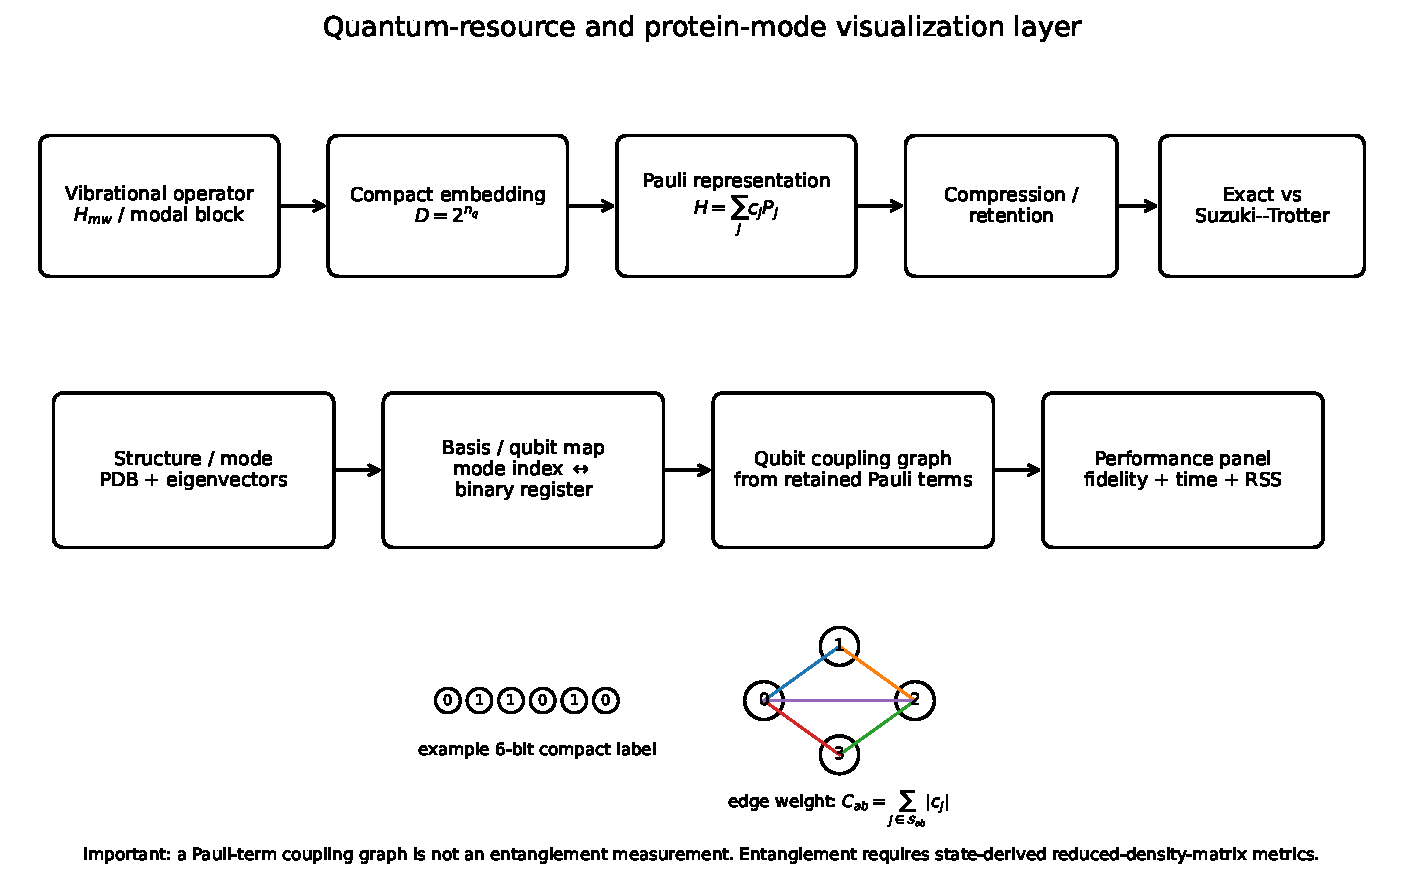
\includegraphics[width=0.94\textwidth]{fig_quantum_viewer_architecture.pdf}
\caption{Proposed resource-aware viewer architecture. Molecular or protein modes are linked to the compact power-of-two register, retained Pauli terms, same-Hamiltonian Suzuki--Trotter validation, and stage-resolved performance telemetry. The qubit network is a Pauli-term coupling graph; it is not an entanglement measurement.}
\end{figure*}

\subsection{Protein-mode interpretation}
The protein extension uses the same distinction between physical coordinates and compact reduced spaces. The existing 1CRN stress test contains 642 atoms and 1926 Cartesian degrees of freedom, while its primary reduced Krylov space has dimension 64 and therefore a six-qubit compact index register. The viewer can associate a selected reduced mode with its structural eigenvector arrows, local basis index, binary register label, and retained operator terms. However, because that stress test did not reproduce the Dense-NMA spectrum with sufficient accuracy, it remains a scalability diagnostic rather than evidence that the reduced six-qubit space replaces complete protein NMA.

For future blockwise full-spectrum protein workflows, the same interface can show a hierarchy
\begin{equation}
\begin{aligned}
\text{protein structure} &\rightarrow \text{mode} \rightarrow \text{block}\\
&\rightarrow \text{local basis index} \rightarrow \text{qubit label}.
\end{aligned}
\end{equation}
provided each displayed quantity is read directly from the validated calculation. A block containing at most 64 modal states requires at most six index qubits, but the full spectrum is represented by the collection of blocks rather than by a single six-qubit register.

\subsection{Scientific guardrails for visualization}
The viewer follows four rules. First, structural animation is generated from stored eigenvectors; exact and Suzuki--Trotter propagation of the same modal basis do not create independent normal-mode shapes. Second, a qubit-coupling graph is derived from retained Pauli terms and must not be relabeled as entanglement. Third, timing plots identify the measured stage and hardware context. Fourth, any hardware-level resource panel remains disabled until gate synthesis, connectivity, state preparation, measurement, and fault-tolerance assumptions are explicitly defined.

These additions make the visualization layer a direct audit surface for the numerical workflow rather than a decorative quantum interface.

\end{document}
